\section*{Resultados}
\subsection*{1. Frecuencia de resonancia para distintos amortiguamientos}
En las Fig. (\ref{fig:I02})---(\ref{fig:I08}) se muestran los regímenes permanentes de 
las oscilaciones forzadas por los voltajes \qtylist{7,30;7,13;7,05;6,95}{\volt}, para cada corriente de amortiguamiento \qtylist{0,2;0,4;0,6;0,8}{\ampere}. Los voltajes empleados
corresponden a la frecuencia de resonancia del péndulo de Pohl para las diferentes
corrientes. Los puntos naranjas en las figuras indican la amplitud de las oscilaciones con
respecto al tiempo.
\begin{figure}[H]
	\centering
	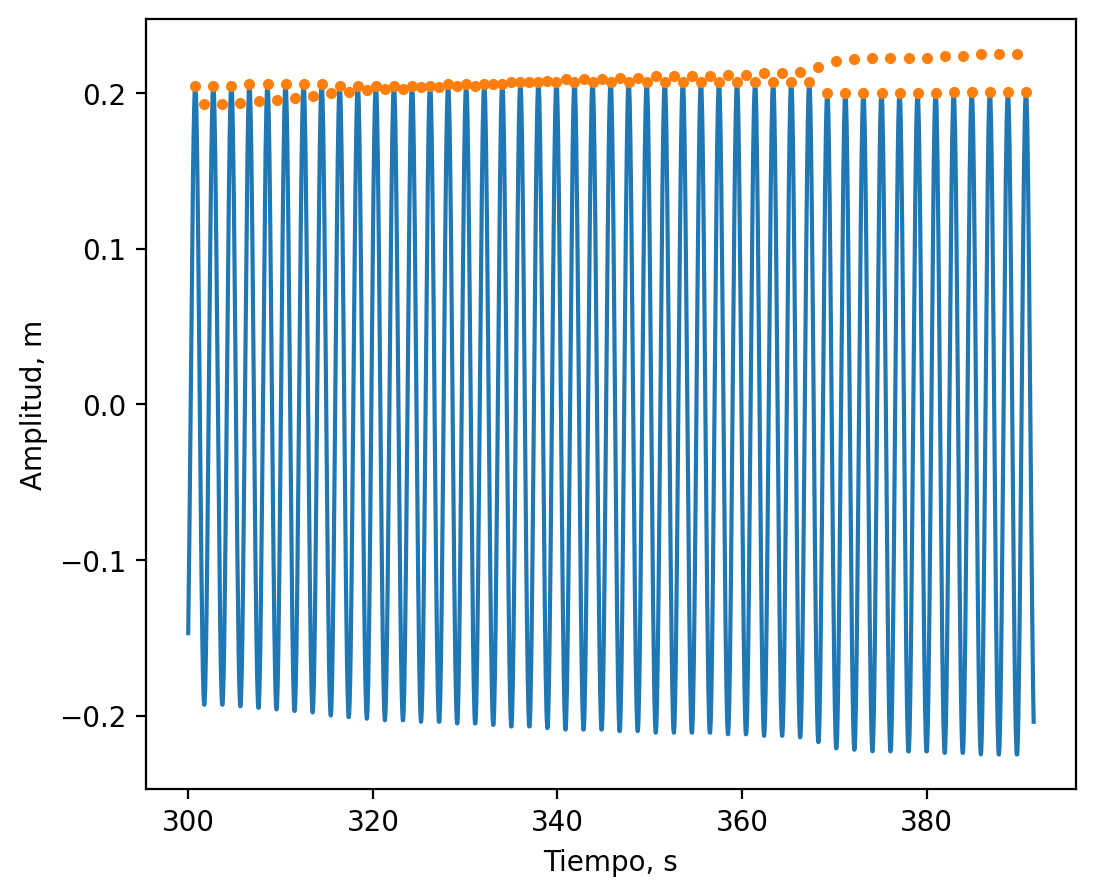
\includegraphics[width=\linewidth]{results/res/I02V73.png}
	\captionof{figure}{Régimen permanente de oscilaciones forzadas. $V$ = \qty{7,30}{\volt},
		$I$ = \qty{0,2}{\ampere}, $\bar{A}_M$ = \qty{0,2072}{\meter}.}
	\label{fig:I02}
\end{figure}

\begin{figure}[H]
	\centering
	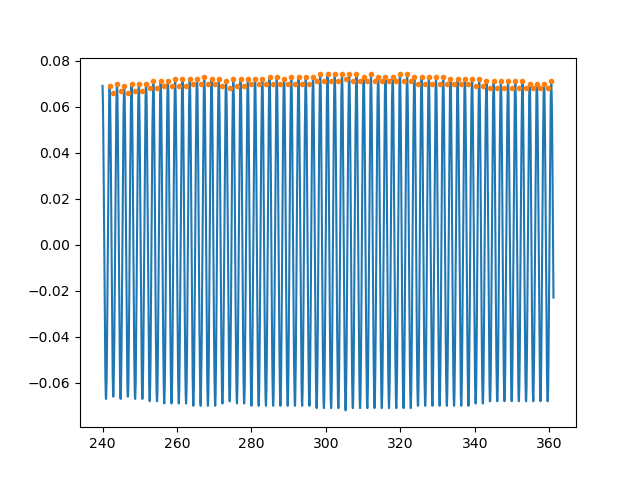
\includegraphics[width=\linewidth]{results/res/I04V713.png}
	\captionof{figure}{Régimen permanente de oscilaciones forzadas. $V$ = \qty{7,13}{\volt}, 
		$I$ = \qty{0,4}{\ampere}, $\bar{A}_M$ = \qty{0,07074}{\meter}.}
	\label{fig:I04}
\end{figure}

\begin{figure}[H]
	\centering
	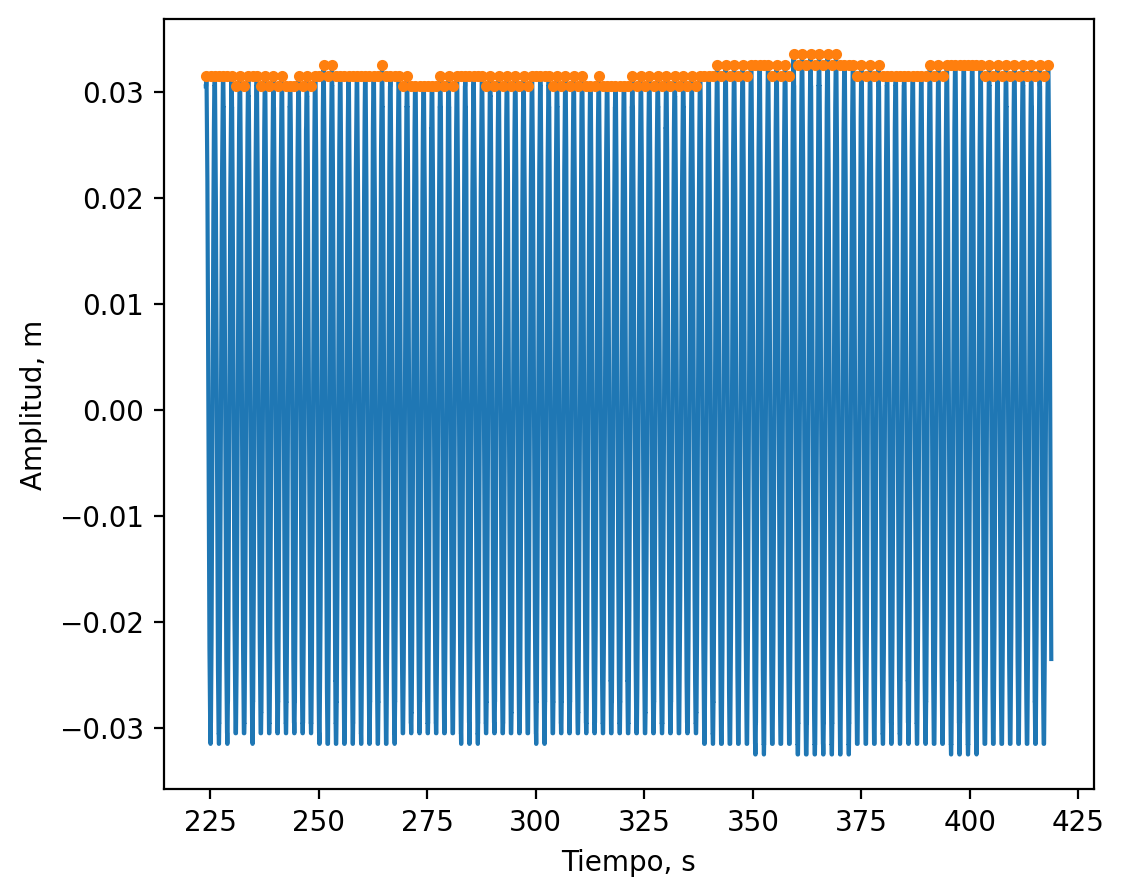
\includegraphics[width=\linewidth]{results/res/I06V705.png}
	\captionof{figure}{Régimen permanente de oscilaciones forzadas. $V$ = \qty{7,05}{\volt},
		$I$ = \qty{0,6}{\ampere}, $\bar{A}_M$ = \qty{0,03154}{\meter}.}
	\label{fig:I06}
\end{figure}

\begin{figure}[H]
	\centering
	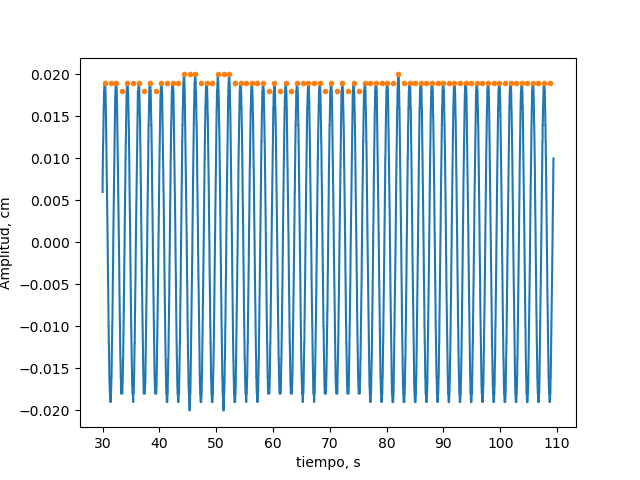
\includegraphics[width=\linewidth]{results/res/I08V695.png}
	\captionof{figure}{Régimen permanente de oscilaciones forzadas. $V$ = \qty{6,95}{\volt},
		$I$ =  \qty{0,8}{\ampere}, $\bar{A}_M$ = \qty{0,01896}{\meter}.}
	\label{fig:I08}
\end{figure}
\vspace{1cm}

En la Tab. (\ref{tab:gammas}) se presentan los valores de la frecuencia de amortiguamiento $\gamma$ y de resonancia $\omega_R$ correspondientes a cada corriente de amortiguamiento y
voltaje impulsor empleado. La frecuencia natural $\omega_0$ establecida para el péndulo fue
de \qty{6,511}{\per\second} y se usó la Ec. (\ref{eq:frecuenciaresonancia}) para determinar el
valor teórico de $\omega_R$. Por otro lado, en el anexo se especifica el proceso empleado
para determinar experimentalmente $\omega_0$, $\gamma$ y $\omega_R$. 

\begin{table}[H]
	\centering
	\captionof{table}{Frecuencia de resonancia y amplitud máxima para las frecuencias de
					amortiguación.}
	\begin{tabular}{c c c c c c}
		\toprule
		 \multirow{2}{*}{$I$, A} & \multirow{2}{*}{$\gamma$, s$^{-1}$} & \multirow{2}{*}{$V$, V} & \multirow{2}{*}{$A_M$, m} & \multicolumn{2}{c}{$\omega_R$, s$^{-1}$} \\
		\cmidrule(l){5-6}
		& & & & Teo. & Exp. \\
		\cmidrule(r){1-2} \cmidrule(l){3-6}
		0,2 & 0,1232 & 7,30 & 0,2072  & 6,509 & 6,423 \\
		0,4 & 0,2220 & 7,13 & 0,07074 & 6,504 & 6,464 \\
		0,6 & 0,3446 & 7,05 & 0,03154 & 6,493 & 6,481 \\
		0,8 & 0,4783 & 6,95 & 0,01896 & 6,476 & 6,338 \\
		\bottomrule
		\label{tab:gammas}
	\end{tabular}
\end{table}

\subsection*{2. Amplitud máxima en función de la frecuencia}

En la Fig. (\ref{fig:amplitudfrecuencia}) se muestra la amplitud máxima $A_M$ de las 
oscilaciones en el régimen permanente con respecto a la frecuencia impulsora empleada 
$\omega_f$, para una corriente de amortiguamiento $I$ = \qty{0,4}{\ampere}. Cada punto en la
figura representa la amplitud registrada en función de la frecuencia del sistema. La curva 
azul es la función de la forma (\ref{eq:amplitudforzada}) que mejor ajusta los puntos. En el
anexo se especifica el proceso empleado para determinar la frecuencia correspondiente a los
voltajes impulsores y la regresión utilizada para establecer la curva.
\begin{figure}[H]
	\centering
	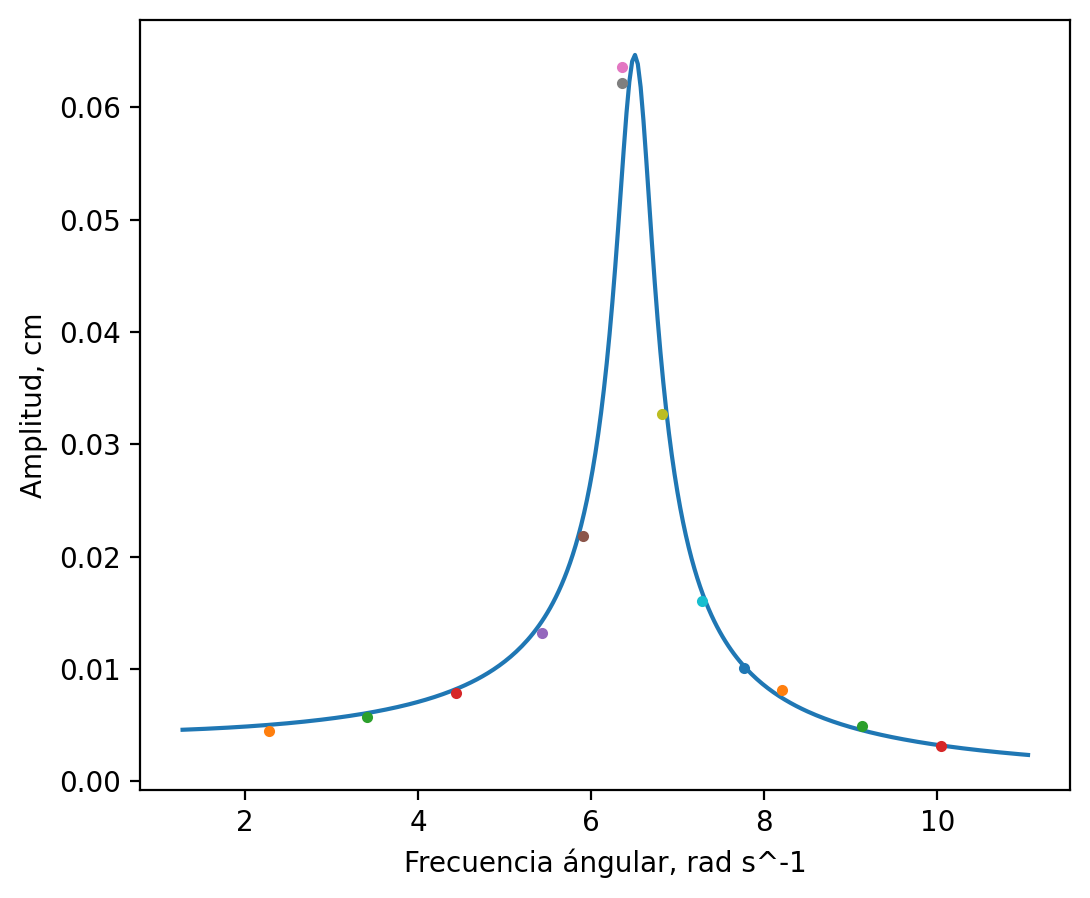
\includegraphics[width=\linewidth]{results/res/reso.png}
	\captionof{figure}{Amplitud máxima en función de la frecuencia para una corriente de
					amortiguamiento de \qty{0,4}{\ampere}. El pico de amplitud ocurre cuando
					$\omega_f=\omega_R=\;$\qty{6,504}{\per\second}.}
	\label{fig:amplitudfrecuencia}
\end{figure}